\chapter{Background}

\label{Chapter2} 

\lhead{Chapter 2. \emph{Background}} 

\section{Native Client}
Native Client (NaCl) can be thought of as a new type of plugin for Google Chrome that allows binary programs to run natively in the web browser. It can be used as a `back end' for a normal web application written in JavaScript, since the binary program will run much faster. A NaCl module can be written in any language, including Assembly, so long as the binary is checked and verified to be safe by the NaCl sandbox \cite{nacl}. However, NaCl provides a Software Development Kit (SDK) that includes a compiler based on gcc that allows developers to compile C and C++ programs into binary that will work directly with the sandbox without further modifications. Thus, writing NaCl-compatible C++ programs is just as easy as writing normal C++ programs. The difference is that the sandboxes disallow unwanted side-effects, including system-calls. Since many applications might want to have these side effects, Native Client provides an Inter-Module Communications service (IMC) which allows modules to communicate with each other. The IMC service allows the use of the Pepper Plug-in API (PPAPI or `Pepper'), a convenient API that is bundled with the SDK. It can be used to do file IO, play audio, and render graphics. The Pepper API also includes the PostMessage functionality that we will use to implement Remote Procedure Calls between JavaScript and NaCl modules.

\subsection{NaCl Modules and the Pepper API}
A native client application consists of the following\cite{nacloverview}:
\begin{description}
  \item[HTML/JavaScript Application] 
  This is where the user interface of the application will be defined, and the   JavaScript here could also perform computations. The HTML file will include   the NaCl module by using an embed tag, e.g. \\
   \verb+<embed src="myModule.nmf" type="application/x-nacl" />+
  \item[Pepper API] 
  Allows the NaCl module communicate with the web browser and use its features.   Provides PostMessage to allow message passing to the JavaScript application.
  \item[Native Client Module] 
  The binary application, which performs heavy computation at native speeds.
\end{description}

\subsection{Communicating with JavaScript using postMessage}
The HTML5 postMessage API was designed to allow web workers to communicate with the main page's JavaScript execution thread. The JavaScript object is copied to the web worker by value. If the object has cycles, they are maintained as long as the cycles exist in the same object. This is known as the structured clone algorithm (need reference). 

In a similar way, postMessage allows message passing to and from NaCl modules. However, sending objects with cycles will cause an error. NaCl allows sending and receiving primitive JavaScript objects (Numbers, Strings, Booleans, null) as well as dictionaries (key-value Objects), arrays, and ArrayBuffers. ArrayBuffers are a new type of JavaScript object based on Typed Arrays \cite{typedarraysw3c} that allows the storing of binary data. Another key difference is that message types need to be converted into the correct type on the receiving end. For example, sending a JavaScript Object should translate into a dictionary type. Type conversions are quite subtle. The JavaScript types are very dynamic in nature. A JavaScript Number object could be an integer, a float, a double, `infinity', exponential, and so on. Sending C++ data to JavaScript is simple since it is converting from a more specific type to a less specific type (e.g. from `int' in C++ to `Number' in JavaScript). But converting from a JavaScript type to a C++ type requires more thought. The C++ Pepper API provides several functions to determine the JavaScript type (e.g. \verb+bool is_double()+), then we can extract and cast the data into our required type, also using Pepper (e.g. \verb+double AsDouble()+). From there, we can use the standard C++ type to perform the required computations.


\section{Remote Procedural Call (RPC)}
RPC is used to uniformly call a procedure that is on a different machine, or on the same machine but on different processes. RPC is implemented on top of a transmission protocol and should work regardless of the communication method we decide to use. For example, we could use TCP/IP for network communications, or any Inter-Process Communication (IPC) method if the caller and callee are on the same machine but in different processes. Normally, remote procedural call implementations would consist of the following steps, as shown in figure \ref{fig:rpc-components}.

\begin{enumerate}
  \item The caller code is written normally, and so is the server code, but the stubs are automatically generated using interface definition files (which we explain later in ...)
  \item When the remote call is made, it calls the user stub which packs the parameters and function call information into a packet.
  \item The packet gets transferred to its destination (either across the network as in figure \ref{fig:rpc-components}, or across the processes on the same machine using IPC). This is done through the RPCRuntime, which is a library that works on both ends (caller and callee) to handle communication details.
  \item The packet is received at the callee end by the RPCRuntime. It is then passed on to the server stub.
  \item The arguments and function call information are unpacked and a normal call is made to the actual procedure.
  \item When the procedure returns, it is passed back to the server stub where it is packed and transmitted back to the caller, which unpacks it and uses the result.
\end{enumerate}

\begin{figure}[!htb]
    \centering
    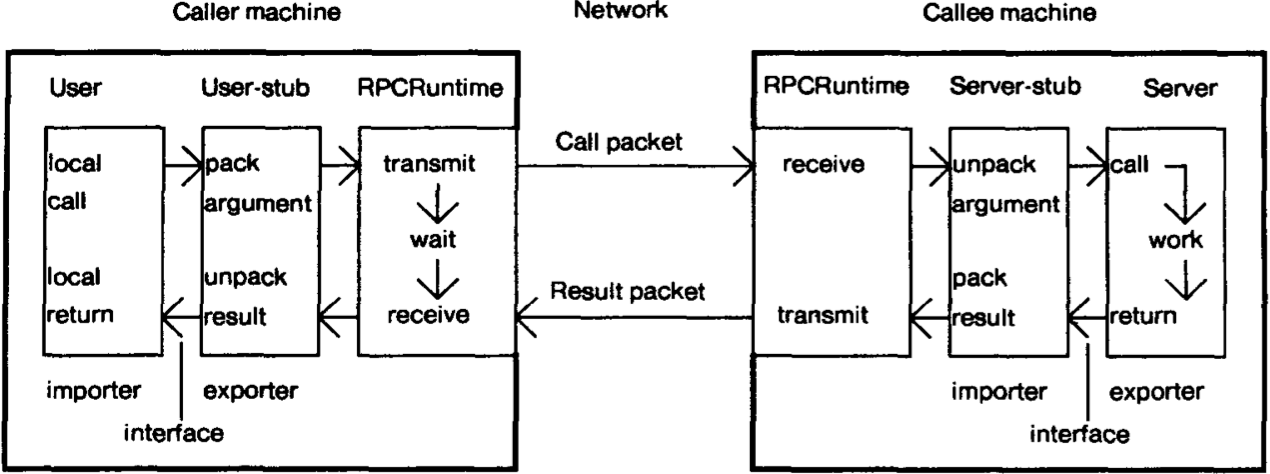
\includegraphics[width=\textwidth]{RPCDiagram_ImplementingRPC_ADBirrell_BJNelson.png}
    \caption{The basic components of an RPC framework, from \cite{birrell1984implementing}}
    \label{fig:rpc-components}
\end{figure}

\subsection{The role of the RPCRuntime}


\subsection{Interface Definition Language}

\section{Inspiration}

